%implementación
%Capitulo consideraciones finales


%porque hacer la prueba?
%cada brueba debe tener una hipotesis o un valor cuantificable

%como se realiza la prueba?
%cuales son los resultados?


%introduccion primero pruebas y luego el caso de studio
Para comprobar el funcionamiento del sistema se realizaron dos pruebas de caja negra y un caso de estudio, las pruebas de caja negra son efectuadas sobre módulos del sistema los cuales tienen datos de entrada, la funcionalidad del modulo y la salida. Mientras que un caso de estudio ayuda a examinar los métodos usados en el sistema.

\section{Captura de Datos}

	De manera similar a como desarrollo el sistema se realizaron las pruebas. Como primer objetivo es realizar el modulo del sistema encargado de la obtención de datos.En esta sección de pruebas se enfoca al tipo de entradas que perite el sistema, para esto se realizo una prueba de caja negra con la cual se establecen criterios de entrada para el tipo de objetos que pueden ser.\\
	
	Esta prueba se buscan los objetos que no son admitidos por el sistema, para esto se uso solo una población representativa de diferentes casos en los que los objetos no serian admitidos.\\
	
	Los objetos no admitidos se dividen por tamaño y material.\\
	
	 \subsection{Por tamaño}
	
	 El sistema solo reconoce objetos que generen al menos veinte puntos, ya que el Kinect da una densidad de puntos cercana a un punto por centímetro a un metro de distancia como se muestra en la figura \ref{fig:coutPoints} y el sistema realiza un filtrado de puntos obteniendo un puto cada dos y medio centímetro. los objetos deben de contar con un área mínima visible al Kinect cincuenta centímetros cuadrados.\\
	 
	 Por el otro lado el objeto no necesita ser visto en su totalidad por el Kinect, pero la clasificación solo se realizara con los datos que puedan ser captados por el Kinect.\\
	 
	
	\begin{figure} [H]
		\centering
		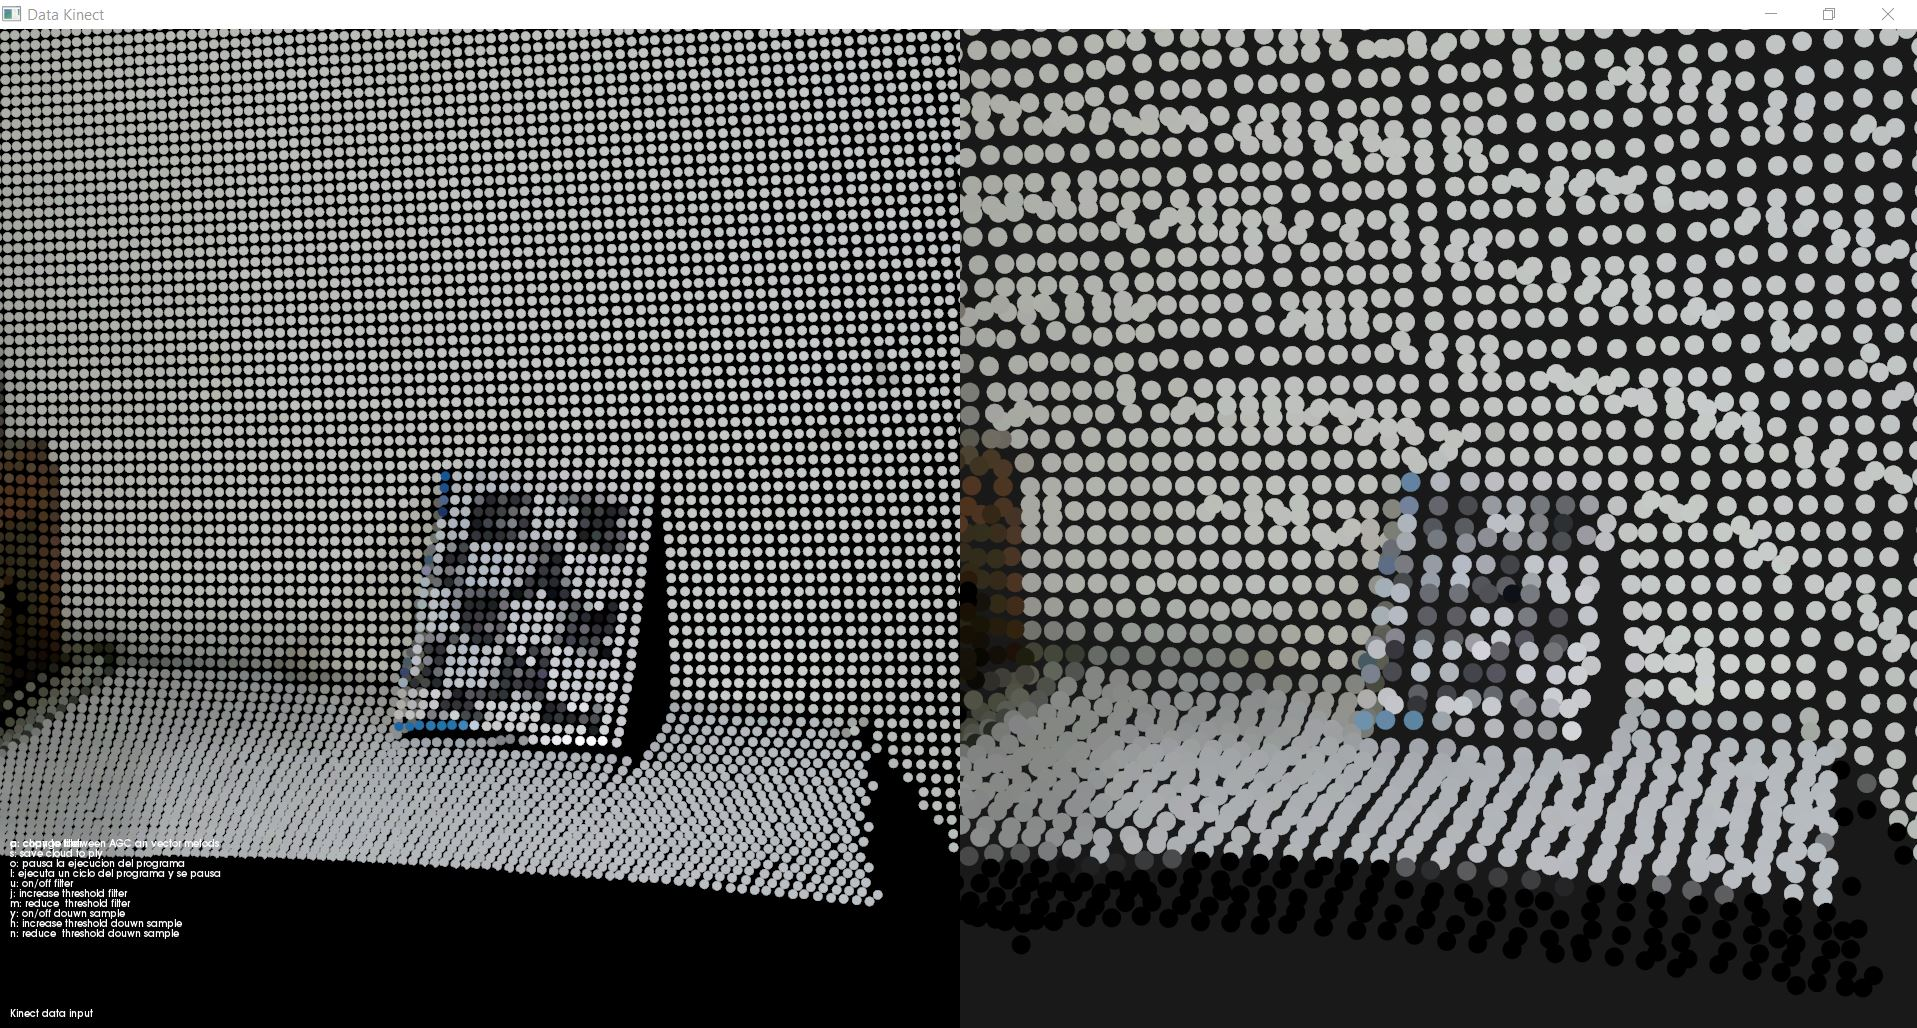
\includegraphics[width=1\textwidth]{03Resultados/imagenes/downsample.JPG}
		\caption{(izq.)Nube de puntos obtenida del Kinect sobre una cuadricula de 5cm,(der.)Nube de puntos resultante luego del filtro de densidad.} 
		\label{fig:coutPoints}
	\end{figure}
	
	
	\subsection{Por material}
	El Kinect al realizar la detección de profundidad usando ToF depende de la luz infrarroja, si un objeto cuanta con un material que absorbe este tipo de luz el Kinect no sera capaz de determinar la nube de puntos. de forma similar ocurre con materiales reflectantes y translucidos.\\
	
\section{Segmentación}

	El modulo encargado de la segmentación se realizo de una prueba de caja negra para encontrar el rengo de trabajo del sistema. Esta prueba engloba tanto la resta de nubes como el agrupamiento de estos.\\
	\subsection{Escenario}
	Ya que para la segmentación se realiza una resta, es necesario capturar el escenario en el cual trabaja el sistema. Este escenario debe cumplir con una serie de lineamientos:
	\begin{itemize}
		\item No debe estar expuesto a la luz del sol o algún otro emisor de luz infrarroja.
		\item El escenario no debe modificarse mientras el sistema este trabajando.
		\item El escenario no debe contener objetos reflectantes o translucidos.
		\item El escenario debe estar separado del Kinect 0.5m y no estar mas alejado de 4.5m.
	\end{itemize}

	\subsection{Objetos}
	\begin{itemize}
		\item El área visible al Kinect debe sobresalir al menos 2.5cm sobre el escenario.
		\item Los objetos deben estar despegados mas de 3cm.
	\end{itemize}
	 
\section{RANSAC}
	A diferencia de las pruebas anteriores en esta se realizara de forma estadística. En esta prueba se engloban dos objetivos particulares: la implementación de un método de clasificación y su modificación para el uso de AGC.\\
	
	El objetivo de esta prueba es el de cuantificar el tiempo, la exactitud y confiabilidad del método elegido así como la modificación realizada con AGC. \\
	
	La precisión del sistema es su capacidad de realizar la clasificación del objeto correctamente, para conocer que tan preciso es el sistema se usan figuras similares a los modelos, se cuenta cada vez que la clasificación es la deseada. al final la precisión $P$ del sistema esta dada por la división de la cantidad de veces que el sistema acertó entre el total de intentos del sistema como se muestra en la ecuación \ref{eq:precision}.
	\begin{equation}
	\label{eq:precision}
	P=\frac{aciertos}{intentos}
	\end{equation}
	
		La exactitud $E$ se entiende por la capacidad del sistema para encontrar el  modelo que representa a la nube de puntos del objeto. Se obtiene con la formula \ref{eq:exactitud} donde $In$ es la cantidad de puntos que coinciden con el modelo y $objeto$ es el total de puntos del objeto.
		 
		 \begin{equation}
		 \label{eq:exactitud}
		 E=\frac{modelo}{objeto}
		 \end{equation}
	
	
	
	Ya que el método RANSAC varia los tiempos dependiendo de que tan cerca este de encontrar un modelo que se ajuste a la nube de puntos esta prueba se realizara usando tres objetos diferentes, estos tienen formas similares a los modelos geométricos que se están usando para conocer que tan confiable y exacto es el método.
	
	Se midieron los tiempos para cada etapa. El proceso que realiza el sistema se divide en ocho etapas:
	%hacer tabla
	DefTiempos
	
	\begin{table}[h]
		\caption{Descripcion de los tiempos del sistema}
		\centering
		\begin{tabular}{ll}
		\hline
		 T1:& La obtención de los datos de sensor Kinect.\\
		 T2:& El filtrado de densidad de puntos.\\
		 T3:& La resta de nubes de puntos.\\
		 T4:& El agrupamiento de los puntos por objeto.\\
		 T5:& Método RANSAC para la esfera.\\
		 T6:& Método RANSAC para el plano.\\
		 T7:& Método RANSAC para el cilindro.\\
		 T8:& Renderizado del resultado.\\
		
		\hline
	\end{tabular}
\label{tab:DefTiempos}
\end{table}
	
	Se realizaron seis pruebas, con tres objetos distintos usando AE y AGC,se colocaron frente al Kinect como en la figura \ref{fig:casoDeESt} en cada una se obtuvieron cien ciclos completos del proceso. La tabla con todos los tiempos para cada prueba se puede consultar en el el apéndice \ref{A:pruebas}.
	
	\begin{figure} [H]
		\centering
		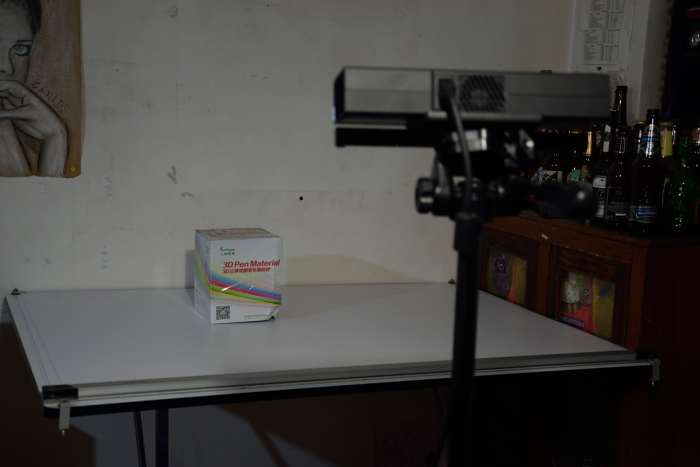
\includegraphics[width=1\textwidth]{03Resultados/imagenes/casoDeEstudio.JPG}
		\caption{Estudio de pruebas} 
		\label{fig:casoDeESt}
	\end{figure}

	La prueba para la esfera de realizo colocando un balón (objeto esférico) frente al Kinect como se muestra en la figura\ref{fig:pruebaEsf}.

\begin{figure} [H]
	\centering
	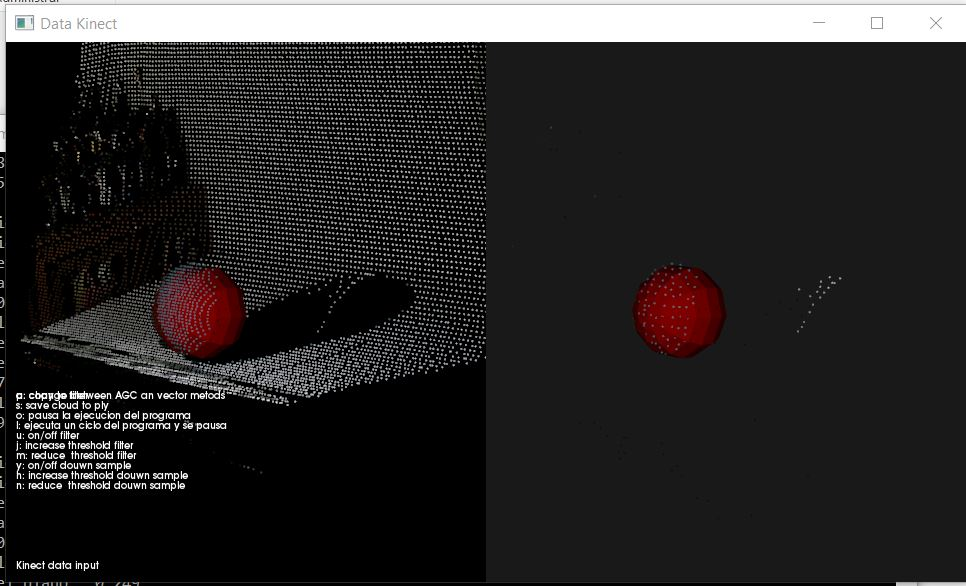
\includegraphics[width=1\textwidth]{03Resultados/imagenes/esfera.JPG}
	\caption{Prueba para la esfera} 
	\label{fig:pruebaEsf}
\end{figure}


La prueba para el plano de realizo colocando un libro (objeto plano) como se muestra en la figura\ref{fig:pruebaPla}.


\begin{figure} [H]
	\centering
	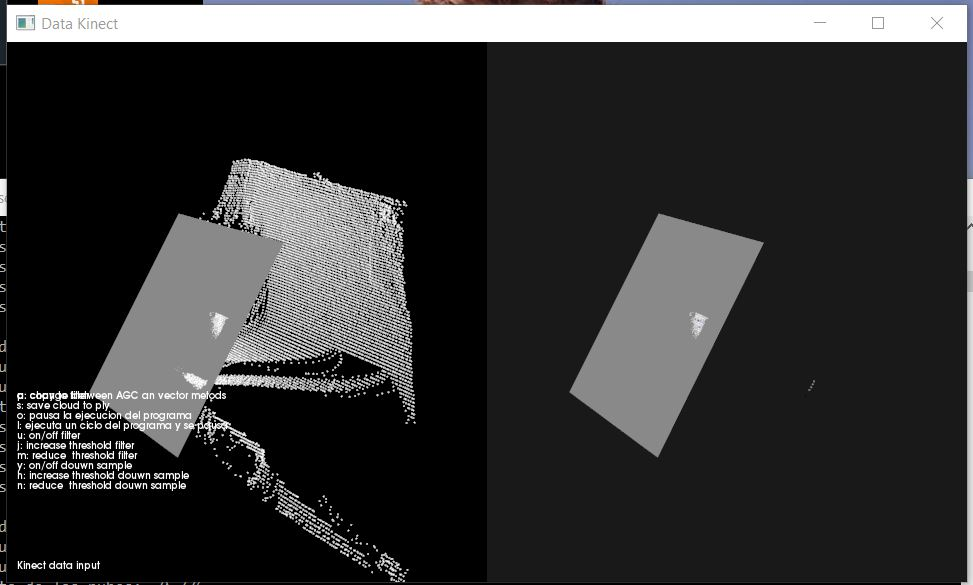
\includegraphics[width=1\textwidth]{03Resultados/imagenes/plano.JPG}
	\caption{Prueba para el plano} 
	\label{fig:pruebaPla}
\end{figure}


La prueba para el cilindro se realizo colocando un  termo cilíndrico como se muestra en la figura\ref{fig:pruebaCyl}.


\begin{figure} [H]
	\centering
	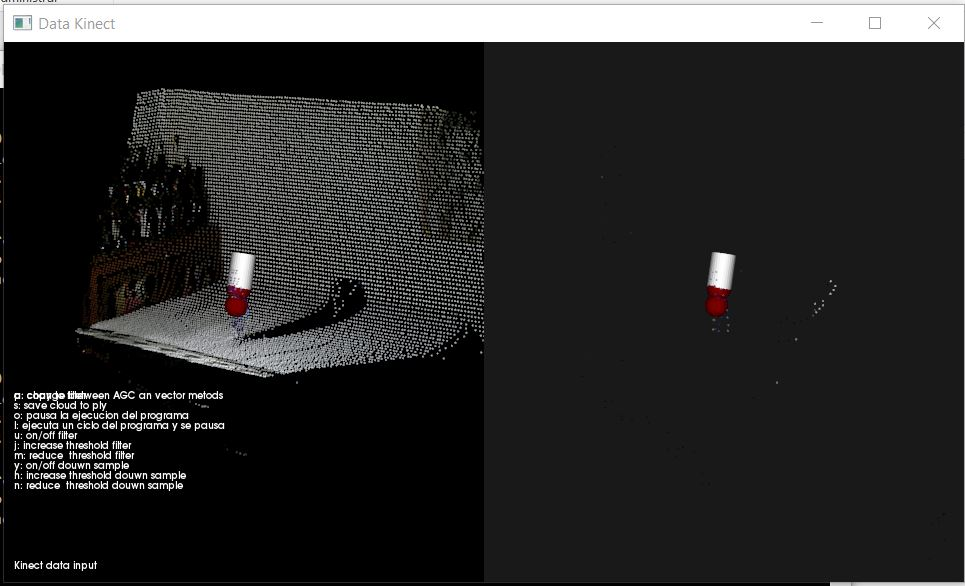
\includegraphics[width=1\textwidth]{03Resultados/imagenes/cilindro.JPG}
	\caption{Prueba para el cilindro} 
	\label{fig:pruebaCyl}
\end{figure}











%recisar la expicacion de las pruebas


%que es la exactitud y la precicion
%como se obtienen


	 
	 
	 
	 
	 
	 
%
%	Uno de los objetivos específicos de este trabajo es el desarrollo de un sistema capaz de obtener datos del sensor Kinect. Esta prueba se diseño para conocer el tiempo requerido por el sensor para realizar el muestreo. El muestreo es independiente al método y en este trabajo se considera una contante.\\
%	
%	El tiempo de muestreo es importante ya que forma parte del ciclo de trabajo y al ser constante el tiempo de respuesta del sistema siempre sera mayor.\\
%	
%	La prueba se lleva acabo sobre el sistema establece la comunicación con el sensor Kinect, crea una nube de puntos con los datos obtenidos, los muestra en pantalla. El tiempo de obtención de datos se mide luego de la conexión con el Kinect hasta antes de que se muestre la nube de puntos en la pantalla.\\
%	
%%	como se muestra en la tabla \ref{tab:planoAGC}.
%%	
%
%\section{Clasificación}
%	Esta prueba se realizo para conocer el tiempo necesario para realizar la clasificación usando RANSAC con AE y que tan precisa y confiable es la clasificación.\\
%	
%	Usando objetos semejantes a las geometrías a clasificar, se colocan uno por vez frente al Kinect para obtener la clasificación del sistema, así como también se calcula que tan representativo es el modelo obtenido comparando el total de puntos en el objeto contra los puntos pertenecientes al modelo.\\
%	
%	
%	
%\subsection{Implementan de AE}
%	La prueba primero se realiza sobe los modelos en AE 
%
%
%\subsection{Implementan de AGC}
%	Para probar el método usando AGC se realiza la misma prueba que en AE para poder coparar los resultados mas adelante.
%	
%\section{Segmentación}
%	Aunque la segmentación se incorporo al sistema desde antes de la clasificación las pruebas de esta no serian relevantes hasta decidir el método de  clasificar a los objetos. ya que la clasificación de un objeto de tarda $t$ tiempo la clasificación se dos seria en $2t$ y así sucesivamente.
	